\subsection{Detecting DDoS Zombie Attacks} \label{subsec:ddos-method}

This experiment deals with detecting zombies which carry out UDP
packet flooding for a DDos attack. In this attack, the compromised
host sends out UDP packets to a victim to consume the victim's
network bandwidth. When the user is absent, legitimate network
traffic rate is low and thus we can potentially detect the malicious
UDP packet flood by observing the traffic rate. However, there could
be background processes that generate network traffic, e.g.
automated updates. Another scenario in our experiment is a
legitimate P2P program.
Unlike the email application, a P2P program can generate network
traffic constantly even when the user is absent. Hence, it is desirable to
derive another feature, instead of the overall rate, to distinguish the
UDP flood attack.

We observe that the UDP flood generates one-way traffic, whereas typical
legitimate processes generate two-way traffic. This motivates us to
consider the net outgoing packet rate $p_{net}$,
\[p_{net} = \max(p_{out} - p_{in},0),\]
\noindent where $p_{out}$ and $p_{in}$ are the outgoing and incoming
packet rate respectively.   We apply CuSum on $p_{net}$, but with a
different threshold $a$ when the user is absent and present.

In addition to $p_{net}$, we also monitor the ratio $r$ of outgoing
packets that are not responded to, \[r=p_{net}/p_{out}.\] We have $0
\leq r \leq 1$ where $r=1$ if the flow has only outgoing packets;
and $r=0$ if $p_{out} \leq p_{in}$. The excess of $p_{net}$ over $a$
is accumulated only if $r \approx 1$.

Fig. \ref{fig:flowrates} compares the maximum net
outgoing packet rate $p_{net}$ and the outgoing packet rate
$p_{out}$ of TCP and UDP network flows when the user is present 
and absent respectively.  A flow is identified by a tuple consisting
of $\langle \mbox{\it local IP}, \mbox{\it remote IP}, 
\mbox{\it transport protocol} \rangle$.
We do not differentiate port numbers as attackers may open
multiple ports to flood the same victim. 
Each flow is monitored for 10 minutes. 
We found this 10 minute observation window to be sufficiently long, because short lived flows last on average only 2 to 3 minutes, 
while flows that last for a long time are likely to
have their traffic rate stabilized within this time.
Fig. \ref{fig:tcpflow_presentrate} shows the distribution of $p_{net}$ and $p_{out}$ of 2,351 non-attack TCP flows active during user presence.
Over 60\% of the flows have the maximum $p_{out}>10$ packets a
minute; whereas less than 5\% of the flows have the maximum
$p_{net}>10$. 
For example, in a sample flow, the maximum $p_{out}$ is 2,443 packets per
minute, but the maximum $p_{net}$ is as low as 10 packets. Fig. \ref{fig:tcpflow_absentrate}, Fig. \ref{fig:udpflow_presentrate} and Fig. \ref{fig:udpflow_absentrate} show the distribution of $p_{net}$ and $p_{out}$ of 980 TCP flows active during user absence, of 9484 UDP flows active during user presence and  1506 UCP flows active during user absence, respectively. They show that $p_{net}$ is more stable a quantity than $p_{out}$ among different flows, regardless of the transport protocol or user presence.

Fig. \ref{fig:ddos} shows the distribution of $p_{net}$ for 13,620 flows.
Fig. \ref{fig:ddos}(a) shows the net outgoing packet rate is close
to 0 for most flows. When the user is present, 35\% of the flows
have $p_{net}=0$; and 80\% flows have $p_{net}$ less than 10 packets
a minute. When the user is absent, 90\% of the flows have
$p_{net}=0$. Fig. \ref{fig:ddos}(b) shows that the difference in
$p_{net}$ when user is present and absent, it can be as large as 600
for some flows, so different upper bounds of normal $p_{net}$ should
be used for user presence and absence and for each flow.

\begin{figure*}[htb]
  \centering
  \subfigure[2351 active TCP flows during user presence]{
    \label{fig:tcpflow_presentrate}
    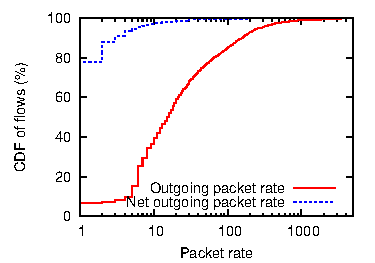
\includegraphics[width=0.45\textwidth]{sensor/tcp-present}}
  \hfill %\hspace{1in}
  \subfigure[980 active TCP flows during user absence]{
    \label{fig:tcpflow_absentrate}
    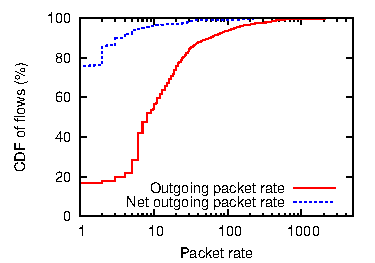
\includegraphics[width=0.45\textwidth]{sensor/tcp-absent}} \\  
  \subfigure[9484 active UDP flows during user presence]{
    \label{fig:udpflow_presentrate}
    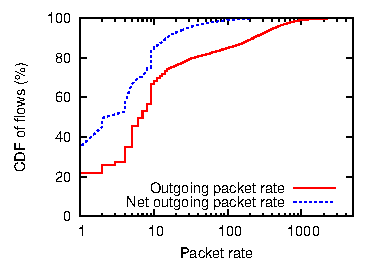
\includegraphics[width=0.45\textwidth]{sensor/udp-present}}
  \hfill %\hspace{1in}
  \subfigure[1506 active UDP flows during user absence]{
    \label{fig:udpflow_absentrate}
    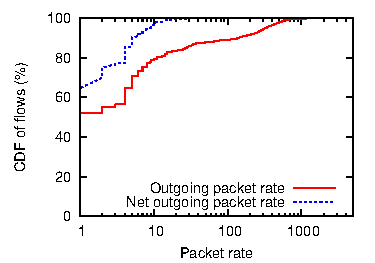
\includegraphics[width=0.45\textwidth]{sensor/udp-absent}}
  \caption{Difference in the outgoing packet rate and the net outgoing packet rate.}
  \label{fig:flowrates}
\end{figure*}

\begin{figure*}[htb]
\centering \subfigure[Distribution of flow net outgoing packet
rates]{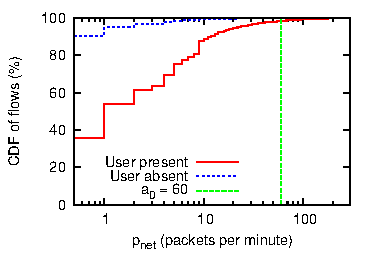
\includegraphics[width=0.48\textwidth]{sensor/net-outrate}}
\subfigure[Difference in the flow rates when user is present and
absent]{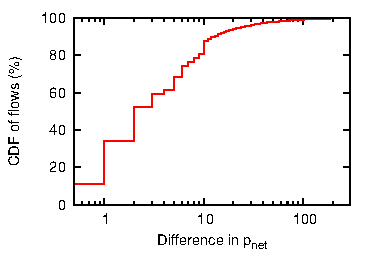
\includegraphics[width=0.48\textwidth]{sensor/net-outrate-diff}}
\caption{Distribution of the maximum net outgoing
packet rate $p_{net}$ with 13,620 TCP and UDP flows, each flow is
observed for 10 minutes during user presence and absence}
\label{fig:ddos}
\end{figure*}

From Fig. \ref{fig:ddos}(a), initializing the upper bound of normal
$p_{net}$ to be $a=60$ packets per minute is sufficient for most
flows. Parameter $a$ can be lowered by examining the online traffic. To
accumulate the excess of $p_{net}$ over $a$, $r$ must be close to 1
and we set it at $0.95$. The threshold to trigger an alarm is
$N=800$ packets, accumulated over 20 minutes. It ensures an attack
flow can be detected if at least 2 UDP packets are sent a second on
average.

\begin{figure}[htb]
\centering
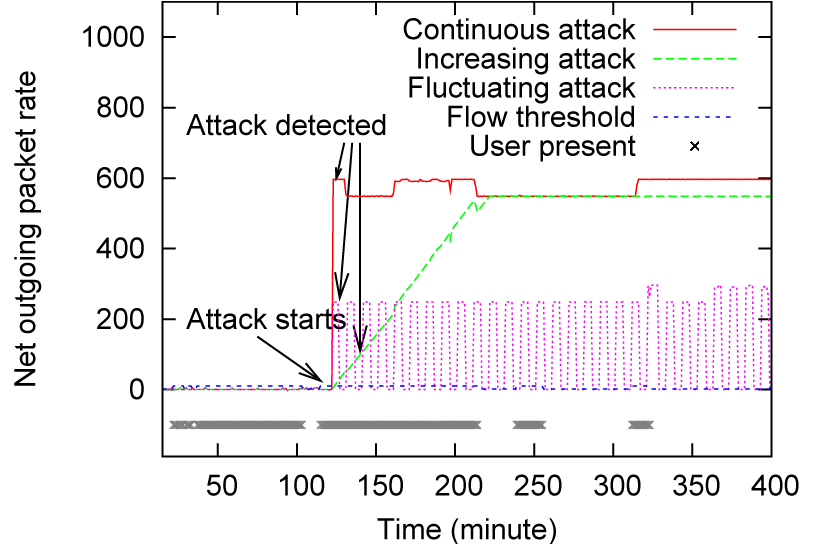
\includegraphics[width=0.7\textwidth]{sensor/ddos-atkflow.png}
\caption{Net outgoing packet rate of the DDoS attack flow in
different attack patterns}
\label{fig:ddos-atkflow}
\end{figure}

\begin{figure}[htb]
\centering
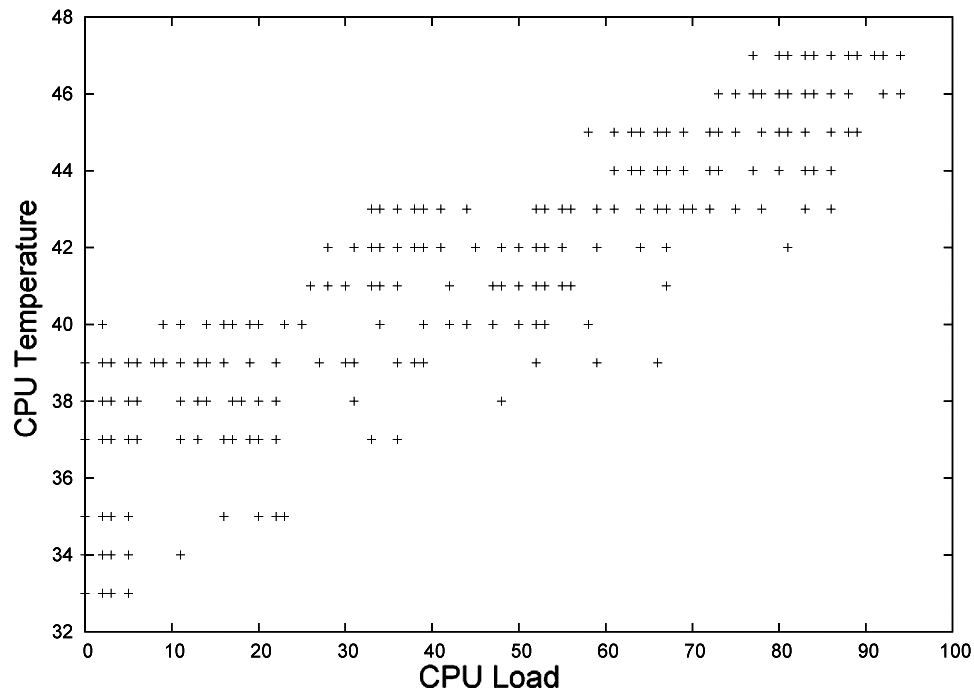
\includegraphics[width=0.7\textwidth]{sensor/load-temp.png}
\caption{Correlation of CPU load and CPU temperature}
\label{fig:temp-cpuload}
\end{figure}

Some non-attack flows have large net outgoing packet rate. However,
they do not cause false alarms, because the outgoing packets are
responded to, or $r$ is not close to 1. In terms of absolute value,
$p_{net}=1278$ is high, but its $p_{out}=2,812$, making $r=0.45$, so
there is 1 response in about 2 packets, the ratio is reasonable and
hence the high net outgoing packet rate is also accepted.

Fig. \ref{fig:ddos-atkflow} shows the net outgoing packet rate
$p_{net}$ of the attack flow under 3 different attack scenarios. The
upper bound $a$ of normal $p_{net}$ is 10 and 2 packets a minute for
user present and absent respectively. These bounds are determined
from analyzing the training data of the flow. The attack starts at
the 125th minute. For the continuous attack, $p_{net}$ sharply
increases to around 600. After 1.36 minutes, the alarm is triggered.
The increasing rate attack increases its attack intensity very
slowly to delay detection. This attack might not be detected if the
detector adapts to the flow rate in near real time. Our approach
detects the attack in less than 18 minutes, long before the attack
reaches its peak rate. The fluctuating attack in Fig. \ref{fig:ddos-atkflow}
constrains the attack intensity, and releases attack traffic in
pulses. This is to avoid detection if average traffic rate or peak
rate is used by the detector. Our approach detects the fluctuating
attack within 3 minutes.

\begin{table}[!t]
  \centering
  \begin{tabular}{|c|c|c|c|}
  \hline
  Detection & Rate & Moving & Changepoint \\
  Algorithm & & Avg (min) & (min) \\
  \hline
  Continuous DDoS  & 1 sec & 1.7  & 1.4   \\
  \hline
  Increasing DDoS & 8.3 min & 17.8  & 17.5   \\
  \hline
  Fluctuating DDoS & 1 sec &  3.6  & 3   \\ [0.5ex]
  \hline
  \end{tabular}
  \caption{Detection time of DDoS attacks of different attack patterns}
  \label{tbl:detect-DDoS}
\end{table}

The DDoS detections using rate and moving average are also set to be relying on the net outgoing packet rate $p_{net}$. The threshold for rate based detection is $T_r = a + N/t$, which is 50 packets per minute or equivalent to $5/6$ packet a second, when user is present. The corresponding threshold for moving average detection is $T_m = 1000$ packets per 20 minutes.
Rate based detection detects continuous and fluctuating DDoS attacks immediately, since $p_{net}$ of the attack flow is high. It detects the increasing rate DDoS attack in 8.3 minutes. 
Depending on the initial state, moving average detects in seconds to minutes the DDoS attacks of different rate patterns. For continuously high rate DDoS attack, the detection time ranges from 1 second to 1.7 minutes. For increasing rate attack, the detection time is the longest, ranging from 15.7 minutes to 17.8 minutes. Whereas for fluctuating rate attack, the detection time ranges from 1 second to 3.6 minutes. The result presented in Table~\ref{tbl:detect-DDoS} shows the worst case. Because in our experiments, the detection has observed a substantially long time of normal behavior before the commence of DDoS attack, the detection is delayed due to the averaging behavior.

%The detection time using moving average detection varies depending on the initial state when the detection starts. The detection time is shortest if the DDoS attack starts before or at the same time as the detection process. Otherwise, the detection will be delayed because moving average combines the previously observed normal behavior and the currently observed high net outgoing packet rate into producing an average.

The effect of user presence information in assisting DDoS attack detection is that it differentiates traffic rates according to user presence, giving a tighter bound on legitimate traffic rate when user is absent, and it makes the detection more effective. 
